  \documentclass[twoside=true, %  doppelseitiger Druck
    DIV=15
    ,% 11 DIV Faktor für Satzspiegelberechnung - muss bei anderen Schriftgrößen als 11pt angepasst werden , sie Doku zu KOMA Script
    BCOR=15mm, % Bindekorrektur
    headinclude=true,
    footinclude=false,
    pagesize,%         write pagesize to DVI or PDF
    fontsize=11pt,%             use this font size
    paper=a4,%          use ISO A4
%    bibliography=totoc,%         write bibliography-chapter to table of contents
    numbers=noenddot
  ]{scrartcl}

\usepackage[utf8]{inputenc}
\usepackage{makeidx}
\usepackage{amsfonts}
%\usepackage[slantedGreek,sc]{mathpazo}  % Schriftart Palatino
\usepackage{lmodern}    % statt mathpazo, falls CM fonts verwendet werden sollen
\usepackage[scaled=.95]{helvet}
\usepackage{courier}
\usepackage[T1]{fontenc}
\usepackage{textcomp}
\usepackage{amsmath}            % standard math notation (vectors/sets/...)
\usepackage{bm}        % standard math notation (fonts)
\usepackage{fixmath}        % standard math notation (fonts)
\usepackage{graphicx}
\usepackage{caption}
\usepackage{subcaption}
\usepackage{scrlayer-scrpage}
% \usepackage{pstool}  % einbinden falls psfrag verwendet werden soll
\usepackage{epstopdf}
\usepackage[ngerman]{babel}
\usepackage{ellipsis}  % Korrigiert den Weißraum um Auslassungspunkte
\usepackage{microtype}  % optischer Randausgleich etc.
\usepackage{acronym}


\usepackage{lipsum} % kann weg, nur zur Generierung von etwas Text im Beispieldokument


\selectlanguage{ngerman}


\deffootnote{1em}{1em}{%
 \makebox[1em][l]{\thefootnotemark}}

\newcommand{\real}{\mathord{\mathrm{I\!R}}}

\begin{document}
\selectlanguage{ngerman}
\def\figdir{figures}
\def\tabledir{tables}

\titlehead{
\raggedleft

\includegraphics[scale=0.7]{\figdir/logo-th-rosenheim-2019_master_quer_2c.eps}
}

\title{
\vspace*{0cm}
Bluetooth Low Energy - Funktionsweise und Einordnung in den Bereich der IOT Kommunikationsprotokolle
}

\author{
Thomas Randl\\
Fakultät für Informatik}

\date{WS 2019/20}

\maketitle

\begin{abstract}
In dieser Arbeit wird der Aufbau und die Funktionsweise der Funktechnik \ac{ble} erläutert. Dabei wird zuerst der Protokollstack im Bezug auf die einzelnen Layer und die \ac{ble} spezifischen Profile betrachtet. Anschließend wird genauer auf die Kommunikation zwischen den einzelnen Verbindungspartnern eingegangen. Dabei wird insbesondere erklärt, welche Schritte notwendig sind um Datenpakete zu übertragen. Des Weiteren wird erläutert, wie der Verbindungsaufbau zwischen den Kommunikationspartnern abläuft und welche Rollen die jeweiligen Partner dabei einnehmen. Nachdem die Funktionsweise erläutert wurde, wird das "`Featureset"' von \ac{ble} erklärt und mit aktuellen \ac{iot} Protokollen verglichen. Anhand der erarbeiteten Informationen wird dann am konkreten Beispiel der "`iBeacons"' erläutert, wie \ac{ble} in der Praxis Anwendung findet.
\end{abstract}

\newpage

\tableofcontents

\newpage

\section*{Abkürzungsverzeichnis} %Abkürzungsverzeichnis 
\begin{acronym}[ECUAF]
	\acro{ble}[BLE]{Bluetooth Low Energy}
	\acro{iot}[IOT]{Internet of Things}
\end{acronym}

%\pagestyle{scrheadings}


\addtokomafont{caption}{\small}


\section{Einleitung}
\label{s:intro}


%%%%%%%%%%%%%%%%%%%%%%%%%%%%%%%%%%%%%%%%%%%%%%%%%%%%%%%%%%%%%%
\subsection{Ein Abschnitt der Einleitung}
\label{ss:intro:abc}

\section{Technische Grundlagen und Implementierungen}
\label{s:grundlagen}

Im folgenden Kapitel wird ein Überblick über die zentralsten \ac{ble} Anwendungen gegeben. Zusätzlich wird die Hardwareebene im Bezug auf die physikalischen Voraussetzungen und die genutzten Frequenzbereiche näher betrachtet. 

\subsection{Beispiele für Implementierungen}
\label{ss:grundlagen:beispiele}

Im einundzwanzigsten Jahrhundert steigt die Verwendung von Geräten, welche drahtlos mit einem Empfangsgerät kommunizieren können. Vor allem die Einführung des Smartphones hat an diesem Punkt die drahtlose Kommunikation vorangetrieben. Nutzer wollen viele Funktionen zur Verfügung gestellt bekommen, um den persönlichen Alltag einfacher gestalten zu können.\\

\noindent Schon vor der Einführung des Smartphones war das Kommunikationsprotokoll "`Bluetooth"' auf Mobiltelefonen verfügbar. Dabei wurde es hauptsächlich zum Datentransfer zwischen zwei Bluetoothfähigen Endgeräten verwendet. Das Hauptproblem, welches der Nutzer dabei erfahren musste, ist, dass diese Form der Datenübertragung sehr viel Zeit in Anspruch genommen hat. Dies lässt sich auf die geringe Datenmenge zurückführen, die pro Paket möglich ist.\\

\noindent Nachdem das Smartphone immer mehr an Beliebtheit gewonnen hat und sich der Begriff des \ac{iot} entwickelt hat, reagierte die Bluetooth \ac{sig}, indem sie ein Protokoll erarbeiteten, welches einen möglichst geringen Stromverbrauch, eine geringe Bandbreite und niedrige Komplexität bietet \cite[Seite 1]{Townsend14:GSB}.\\

\noindent Mit der Einführung von \ac{ble} kam die Möglichkeit kleine Datensignale zwischen Geräten auszutauschen. Ein aktuell sehr bekanntes Beispiel sind dabei sogenannte "`Smartwatches"'. Diese bieten neben der Möglichkeit die Uhrzeit bereitzustellen viele weitere Funktionen, wie beispielsweise die Steuerung von Telefongesprächen, oder die Fernsteuerung der Musikwiedergabe. Der Nutzer erhält durch ein derartiges Gerät die Möglichkeit, sein Smartphone in gewissen Bereichen fernzusteuern.\\

\noindent Beinahe jeder Mensch in der heutigen Zeit besitzt und nutzt ein Smartphone. Jedes Smartphone ist dabei mit einer Bluetoothschnittstelle ausgestattet. Dieser Sachverhalt liefert die Möglichkeit, nicht nur eine "`Smartwatch"' mit dem Smartphone zu verbinden, sondern jegliches Empfangsgerät, welches der Nutzer benötigen könnte. Besonders beliebt sind dabei Fitnessgeräte, die dem Nutzer Informationen über sein Fitnesslevel liefern.\\

\noindent Allerdings liefert der Sachverhalt, dass beinahe jeder Nutzer Bluetooth nutzt auch andere "`Usecases"'. Mit sogenannten "`Beacons"' (siehe Kapitel \ref{s:ibeacon}) kann man beispielsweise mit einem Smartphone Informationen von einem oder mehreren "`Beacons"' erfassen und in einer App oder im Browser gesammelt aufbereitet anzeigen. Ein "`Beacon"' ist ein \ac{ble} Gerät, welches ausschließlich Informationen sendet. So kann man beispielsweise in einem Raum mit mehreren solchen Geräten stehen und Informationen über verschiedene Lebensmittel, oder deren Preise erhalten. Mit dieser Möglichkeit kann ein Nutzer noch besser und zielgerichteter mit sachdienlichen Informationen versorgt werden.\\

\noindent Sollte man die Absicht haben, ein eigenes Gerät zu entwickeln, welches mittels \ac{ble} kommuniziert, gibt es mehrere Anbieter für Hardwarekomponenten für verschiedene Anwendungsfälle. Besonders nennenswert sind dabei die Firmen "`Nordic"' und "`Texas Instruments"'.\\

\noindent Die Firma "`Nordic"', welche Kompononenten für verschiedenste Kommunikationsprotokolle anbietet, ist Mitglied bei der Bluetooth \ac{sig} und hat einen signifikanten Beitrag zum fortschritt von \ac{ble} beigetragen. Sie war auch eine der ersten Firmen, die günstige \ac{ble} Komponenten auf den Markt gebracht haben \cite[Seite 75]{Townsend14:GSB}.\\

\noindent Die Firma "`Texas Instruments"' hingegen war als erstes dazu in der Lage, ein \ac{ble} fähiges Peripheriegerät auf den Markt zu bringen. Zusätzlich ist "`Texas Instruments"' als einiger Anbieter "`Feature complete"'. Das heißt, dass die Geräte den kompletten Funktionsumfang des \ac{ble} Stacks anbieten \cite[Seite 79]{Townsend14:GSB}.\\ 

\subsection{Hardware}
\label{ss:grundlagen:hardware}

  

\subsection{Frequenzbereich}
\label{ss:grundlagen:frequenz}

Da \ac{ble} ein Teil des Bluetoothstacks ist, sind die physikalischen Eigenschaften, die sowohl hinter Bluetooth Klassik, als auch \ac{ble} stecken identisch. Der Frequenzbereich, indem Bluetooth sendet ist dementsprechend auch der selbe. Allerdings gibt es einen Unterschied, was die Kanäle angeht, in denen gesendet wird.\\

\noindent Der Frequenzbereich in dem sich Bluetooth bewegt liegt zwischen 2,4GHz und 2,4835GHz auf dem \ac{ism} Band \cite[Seite 16]{Townsend14:GSB}. Diesen Bereich teilt sich Bluetooth mit einigen anderen Kommunikationsprotokollen, weshalb es zwischen den Protokollen zu Kollisionen bei der Übertragung kommen kann. Aus diesem Grund teilt Bluetooth seinen Bereich in mehrere Kanäle auf. Bei Bluetooth Klassik ist der Frequenzbereich in insgesamt 79 Kanäle unterteilt \cite[Seite 410]{Sauter18:GMK}. \ac{ble} teilt den Bereich allerdings nur in 40 Kanäle auf \cite[Seite 16]{Townsend14:GSB}. Daraus resultiert, dass die Kanäle bei \ac{ble} doppelt so groß sind wie bei Bluetooth Klassik. Der Grund für diese Kanalunterteilung ist das sogenannte "`Frequency Hopping"', welches unter Kapitel \ref{sss:funktionsweise:physical} näher betrachtet wird.\\  

\section{Funktionsweise Bluetooth Low Energy}
\label{s:funktionsweise}
beispielsweise
Im nachfolgenden Kapitel wird nun auf die Softwareseitigen Aspekte des \ac{ble} Stacks eingegangen. Dabei finden die Architektur und die Kommunikation besondere Beachtung. Zusätzlich wird ein Überblick geboten, welche Möglichkeiten diese Technologie dem Nutzer bietet.\\  

\subsection{Protokollstack}
\label{ss:funktionsweise:protokollstack}

In Abbildung \ref{FIG:protokollstack} ist der Protokollstack von \ac{ble} zu sehen. Dabei sind die drei Ebenen "`Controller"', "`Host"' und "`Application"' zu erkennen. Auf der untersten Ebene liegt der "`Controller"', in welchem das "`Physical Layer"' und das "`Linked Layer"' enthalten sind. Zwischen "`Host und "`Controller"' liegt das sogenannte \ac{hci}, welches die Schnittstelle zwischen den beiden Kommunikationspartnern darstellt. Im "`Host"' wiederum befinden sich sämtliche Protokolle und Profile, die notwendig sind, um Kommunikation zu ermöglichen. An der Spitze des Protokollstacks befindet sich die "`Applikation"' in der die Logik und Nutzerschnittstelle des aktuellen Anwendungsfalls liegt \cite[15]{Townsend14:GSB}. Wie diese einzelnen Komponenten funktionieren und untereinander kommunizieren ist in den nachfolgenden Abschnitten erläutert.\\  
 
\begin{figure}[h]
\centering
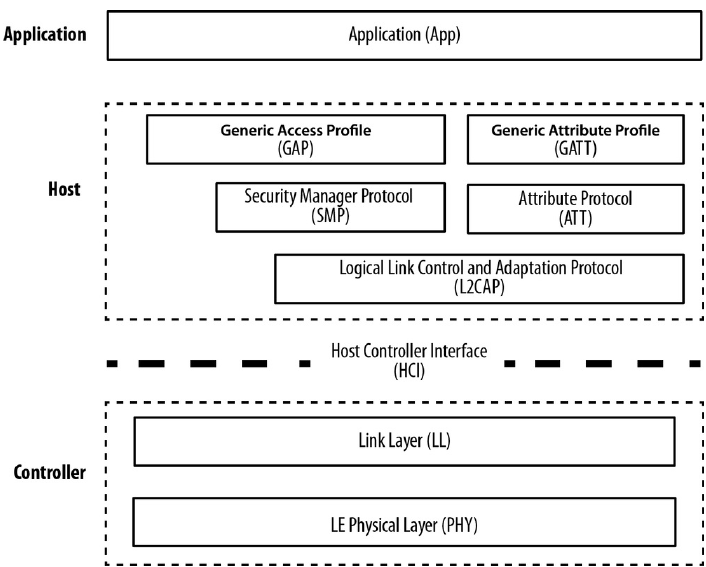
\includegraphics[width=\linewidth]{\figdir/BLE_Protokolstack}
\caption{\ac{ble} Protokollstack \cite[Seite 16]{Townsend14:GSB}}
\label{FIG:protokollstack}
\end{figure}

\subsubsection{Physical Layer}
\label{sss:funktionsweise:physical}

Das sogenannte "`Physical Layer"' bildet die Basis der Kommunikation bei einer Großzahl von Gerätearchitekturen. In dieser Schicht werden digitale Signale, also Bitfolgen, in analoge Signale umgewandelt. Dieser Vorgang wird zum Senden von Nachrichten über eine physikalische Schnittstelle benötigt. Die Rückübersetzung in eine digitale Bitfolge wird ebenfalls im "`Physical Layer"' erledigt \cite[Seite 16]{Townsend14:GSB}. Als physikalisches Medium bieten sich dabei eine Vielzahl von Möglichkeiten, wie unter anderem Magnetismus, Strom, oder Licht \cite[Seite 95 - 101]{Tanenbaum14:CN}.\\

\noindent Bei \ac{ble} ist die besagte physikalische Schnittstelle die Luft. \ac{ble} nutzt in dieser wie in Kapitel \ref{ss:grundlagen:frequenz} erläutert einen definierten Frequenzbereich um Nachrichten zu übertragen. Dabei belegt \ac{ble} nur einen sehr kleinen Bereich des verfügbaren Spektrums. Insgesamt deckt der verfügbare Frequenzbereich in etwa einen Bereich von 30.000GHz ab. In ihm werden unter anderem Radiowellen, Fernsehübertragungen, Satellitensignale und viele weitere Nachrichtenpakete transportiert \cite[Seite 107]{Tanenbaum14:CN}. Im Frequenzbereich in dem \ac{ble} übertragen wird befinden sich trotz des großen Spektrums einige konkurrierende Technologien, wie beispielsweise "`Wireless LAN"' \cite[Seite 17]{Townsend14:GSB}. Aus diesem Grund verwendet Bluetooth im allgemeinen das sogenannte "`Frequency Hopping Spread Spectrum"'. Dafür wird der verfügbare Frequenzbereich im Fall von \ac{ble} in 40 Kanäle aufgeteilt. Von diesen werden die letzten drei Kanäle zum "`Advertisment"', also zur Bekanntmachung, verwendet. Über diese gibt sich ein Gerät zu erkennen, welches bereit zum Verbinden ist. Ein suchendes Gerät wiederum überprüft ausschließlich diese drei Kanäle nach verfügbaren Geräten. Die restlichen 37 Kanäle werden anschließend für die Übertragung verwendet. Dabei wird zu Beginn des Datenaustausches eine Sprungfrequenz vereinbart, welche daher für jede neue Verbindung voneinander abweicht. Nachdem die Verbindungsinformationen vereinbart wurden, beginnt der Datenaustausch. In Formel \ref{eq:ble:frequencyhopping} ist zu erkennen, wie die Verbindungspartner gegenseitig abstimmen, in welchen Kanal sie als nächstes wechseln werden. Diese Berechnung führt jedes Gerät unter Berücksichtigung der vereinbarten Verbindungsinformationen selbst aus \cite[Seite 17]{Townsend14:GSB}. 
\begin{equation}
\label{eq:ble:frequencyhopping}
Kanal = (aktueller Kanal + Sprungfrequenz) \mod 37
\end{equation}
Sollte dennoch ein Paket bei der Übertragung verloren gehen, wird dieses nach sofortigem Kanalwechsel erneut übertragen. Sollte es mehrfach zu Problemen mit einem oder mehreren Kanälen kommen führt Bluetooth eine Kanalabschätzung durch. Dabei wird eine "`Channel Bitmap"' mit Kanälen erzeugt, welche eine hohe Interferenz aufweisen. Diese werden anschließend für die laufende Verbindung gesperrt. Um festzulegen, ob ein Kanal blockiert ist, gibt es die folgenden drei Möglichkeiten:

\begin{itemize}
	\item[1.]{\ac{rssi}}
	\item[2.]{Eine hohe Packetfehlerrate}
	\item[3.]{Informationen eines Endgerätes mit Zugriff auf konkurrierende Funktechnologien}
\end{itemize}       

\noindent Welche dieser Optionen verwendet wird ist allerdings vom Standard nicht vorgeschrieben und kann deshalb selbstständig definiert werden \cite[Seite 411]{Sauter18:GMK}.\\

\noindent 

\subsubsection{Linked Layer}
\label{sss:funktionsweise:linked}

Das "`Linked Layer"' liegt in der Architektur direkt auf dem "`Physical Layer"'. Dabei stellt es entweder die zu sendenden Daten bereit, oder verarbeitet die vom "'Physical Layer"' empfangenen. Um dies bewerkstelligen zu können, werden Nachrichten nach einem definierten Schema in sogenannte "`Frames"' gepackt. Diese enthalten zusätzlich zur eigentlichen Nachricht wichtige Informationen bezüglich des Paketes. Mit diesen kann unter anderem überprüft werden, ob es zu Fehlern bei der Übertragung gekommen ist, indem man eine "`CRC Checksumme"' bildet \cite[Seite 194]{Tanenbaum14:CN}.\\

\noindent Das "`Linked Layer"' wird bezüglich der zu verarbeitenden Daten für jede Kommunikationsart angepasst. Im Fall von \ac{ble} gibt es daher einige Eigenschaften, welche sich von anderen Protokollen unterscheiden. Zum einen gilt es zu beachten, dass die \ac{ble} Kommunikation auf einem Nachrichtenaustausch beruht, der sehr schmale Zeitfenster aufweist in denen Nachrichten gesendet werden können. Aus diesem Grund wird das "`Linked Layer"' hier weitestgehend von den oberen Protokollschichten getrennt und kommuniziert nur über das \ac{hci} mit diesen. Daraus Folgt wiederum, dass das "`Linked Layer"' sehr schnell in der Verarbeitung von Daten ist \cite[Seite 17f]{Townsend14:GSB}.\\

\noindent Jedes \ac{ble} Gerät verfügt über eine eindeutige Adresse. Diese ist Aufgebaut wie eine "`MAC Adresse"'. Diese Adresse kann das Gerät bei einem "`Advertisement"' versuch broadcasten und andere Geräte können sich dann mit dieser Koppeln. Der Verbindungsprozess hat also verschiedene Rollenverteilungen die von der auszuführenden Aktion des Gerätes abhängen. So ist ein Gerät, welches auf einen Verbindungspartner wartet, ein "`Advertiser"'. Das bedeutet, dass dieses Gerät dauerhaft auf den Advertisementkanälen seine Adresse und andere wichtige Informationen für einen potentiellen Verbindungspartner preisgibt. Der potentielle Verbindungspartner in diesem Fall hat die Rolle des "`Scanners"' inne. Das bedeutet, dass er gerne eine Verbindung eingehen würde. Um dies zu tun überprüft er die drei Advertisementkanäle nach "`Advertisern"'. Diese werden dann beispielsweise dem Nutzer in einer Liste angezeigt. Hier werden nur Geräte angezeigt, welche noch keine aktive Verbindung aufweisen. Das liegt daran, dass die Verbindungspartner bei einer erfolgten Verbindung ihre Rollen ändern. Der "`Scanner"' wird zum "`Master"' der Verbindung und steuert diese. Der "`Advertiser"' wiederum wird zum "`Slave"' der Verbindung und folgt den Anweisungen des "`Masters"' bezüglich des Timings. In der Regel handelt es sich bei "`Slave"' Geräten um einfache Geräte mit niedrigen Funktionalitäten, wohingegen der "`Master"' meist ein leistungsstärkeres Gerät darstellt \cite[Seite 18f]{Townsend14:GSB}.\\  

\noindent Bei \ac{ble} tritt gegenüber dem normalen Bluetoothprotokoll die Besonderheit auf, dass es nicht zwangsläufig zu einer Verbindung zwischen "`Master"' und "`Slave"' kommen muss. Geräte wie "`Beacons"' beispielsweise arbeiten nur auf den Advertisementkanälen und senden dauerhaft Informationen an alle \ac{ble} Geräte in Reichweite \cite[Seite 13]{Gast14:BPA}. Näheres hierzu findet sich unter Kapitel \ref{s:ibeacon}.\\


\noindent Wenn ein Gerät auf der Suche nach einem Verbindungspartner ist, hat es zwei Möglichkeiten. Zum einen kann es einen passiven Scan auf die Advertisementkanäle durchführen, bei dem der "`Advertiser"' nicht mitbekommt, dass er erfasst wurde. Zum anderen kann ein aktiver Scan durchgeführt werden, mit dem eine aktive Anfrage an das zur Verfügung stehende Gerät gesendet wird, um weitere Informationen einzuholen und das Gerät über einen potentiellen Verbindungspartner zu informieren. Die Nachricht, welche bei einem aktiven Scan an den "`Scanner"' gesendet wird enthält drei zentrale Informationen:
\begin{itemize}
	\item[1.]{Die Möglichkeit einer Verbindung (Ja/Nein)}
	\item[2.]{Die Möglichkeit einen aktiven Scan durchführen zu können (Ja/Nein)}
	\item[3.]{Die Information, ob der "`Advertiser"' ein "`Broadcaster"' ist (Ja/Nein)}
\end{itemize}           
Sollte der "`Advertiser"' ein "`Broadcaster"' sein ist es erlaubt, nutzerspezifische Daten in den Nachrichten auszutauschen. In allen anderen Fällen werden hier ausschließlich verbindungsspezifische Daten ausgetauscht \cite[Seite 20f]{Townsend14:GSB}.\\

\noindent Für den Fall, dass der "`Advertiser"' kein "`Broadcaster"' ist, ergibt sich die Möglichkeit eine Verbindung aufzubauen. Um das zu bewerkstelligen sendet der "`Scanner"' eine Verbindungsanfrage. Eine Verbindung in \ac{ble} steht für eine Abfolge von Verbindungsevents, bei denen Nachrichten ausgetauscht werden. Der "`Scanner"' nimmt nun die Rolle des "`Masters"' an und legt in der Verbindungsanfrage drei grundlegende Eckpunkte fest. Zum einen die Zeitspanne, die vergeht, bis ein neues Verbindungsevent stattfindet. Je größer diese Zeitspanne ist, desto weniger Energie wird verbraucht. Ein weiterer Punkt ist die Anzahl der Verbindungsevents, welche der "`Slave"' überspringen darf, ohne die Verbindung zu beenden. Der letzte Punkt ist die Zeit, die vergehen darf, bis ein Timeout ausgelöst wird \cite[Seite 21f]{Townsend14:GSB}.\\ 

\noindent Im "`Linked Layer"' wird die maximale Paketgröße festgelegt. In älteren Versionen von \ac{ble} lag die Payloadgröße, welche jedes Nachrichtenpaket maximal beinhalten konnte, bei 27 Byte. In Abbildung \ref{FIG:payload} ist der Aufbau eines Nachrichtenpaketes dargestellt. Besonders wichtig ist hierbei die Größe der Payload. Bezüglich dieser kann man erkennen, dass sich diese mit Version 4.2 auf 251 Bytes erhöht hat. Das wurde durch die Einführung der "`Data Length Extension"' ermöglicht. Dieses Upgrade schafft die Voraussetzungen dafür, Nachrichten in weniger Zeit übertragen zu können, da mehr Informationen in ein Paket passen \cite{Gupta:WWW}.\\   

\begin{figure}[h]
	\centering
	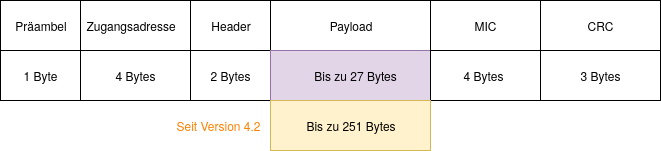
\includegraphics[width=\linewidth]{\figdir/Payload}
	\caption{Aufbau eines Nachrichtenpaketes bei \ac{ble}}
	\label{FIG:payload}
\end{figure}

\noindent Sollte ein Paket fehlerhaft übertragen werden, wird dieses mittels der CRC Checksumme entdeckt und dieses Paket wird so lange wiederholt, bis die Checksumme korrekt ist. Dabei gibt es keine Obergrenze für die Anzahl an Wiederholungen \cite[Seite 23]{Townsend14:GSB}.\\

\subsubsection{Protokolle}
\label{sss:funktionsweise:protocoll}

In Abbildung \ref{FIG:protokollstack} ist zu erkennen, dass sich zwischen den Schichten des "`Controllers"' und des tatsächlichen "`Hosts"' das \ac{hci} befindet. Dessen Zweck zeigt sich hauptsächlich bei leistungsstarken Geräten. Diese bieten den Vorteil, dass komplexe Funktionen ausgeführt werden können. Da \ac{ble} allerdings einige Funktionalitäten aufweist, welche für die Kommunikation essenziell sind und möglichst schnell abgehandelt werden müssen, werden diese zumeist in einen separaten Hardwarechip ausgelagert. Somit liegt der "`Controller"' Teil des Protokollstacks in der Regel nicht auf dem Prozessor. Die eigene Implementierung und die dafür benötigten Protokollschichten liegen allerdings aufgrund der Leistung auf der CPU. Einzige Ausnahme davon sind kleine Geräte, welche nicht viel Leistung benötigen und nur einfache Funktionen mit \ac{ble} ausführen. Bei diesen kann es sehr wohl vorkommen, dass der komplette Protokollstack auf einem einzigen Hardwarechip lokalisiert ist \cite[Seite 24]{Townsend14:GSB}. Im Folgenden wird nun erläutert welche Schichten sich im "'Host"' befinden und es wird auf deren Funktionen eingegangen.\\  

\noindent Die Basis der Protokoll bietet das \ac{l2cap}. Dessen Hauptaufgabe ist es, zu gewährleisten, dass die Pakete, welche von den höheren Schichten versendet werden wollen, den Kriterien der "`Controller"' Schichten entsprechen. Ebenfalls verarbeitet es die empfangenen Pakete der unteren Schichten. Dabei liegt das Hauptaugenmerk auf der Fragmentierung der Pakete in die entsprechenden Pakete. Wie unter Abschnitt \ref{sss:funktionsweise:linked} erläutert kann \ac{ble} nur eine begrenze Anzahl an Bytes pro Paket versenden. Das \ac{l2cap} sorgt dafür, dass Nachrichten entsprechen aufgeteilt an das Linked Layer übergeben werden \cite{TI:WWW}.\\

\begin{figure}[h]
	\centering
	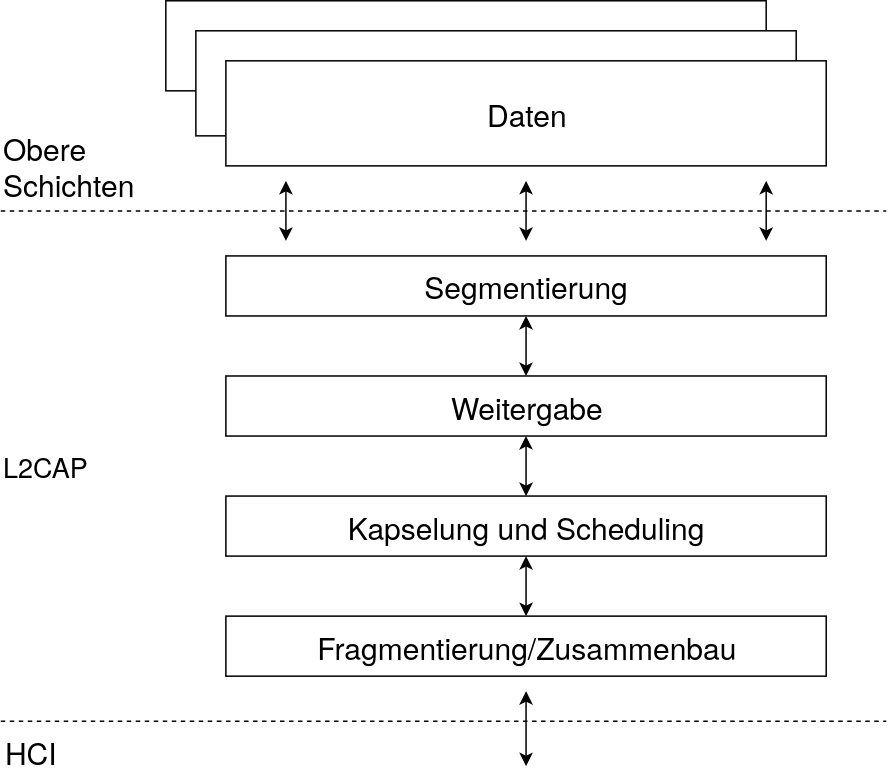
\includegraphics[width=0.5\linewidth]{\figdir/L2CAP}
	\caption{Funktionsebenen des \ac{l2cap} \cite{TI:WWW}}
	\label{FIG:l2cap}
\end{figure}

\noindent Zusätzlich fungiert das \ac{l2cap} als Protokoll Multiplexer. Das bedeutet, dass es mehrere Schichten über sich akzeptiert und diese in das Standard \ac{ble} Paketformat bringt \cite[Seite 25]{Townsend14:GSB}. In Abbildung \ref{FIG:l2cap} sind die einzelnen Arbeitsschritte und deren Zusammenhang dargestellt. Daraus geht hervor, dass jedes Datenpaket vier Bereiche durchlaufen muss, um von den oberen Schichten in das \ac{hci} zu gelangen. In die andere Richtung werden die selben Ebenen durchlaufen. Dementsprechend werden hier Pakete segmentiert, bevor sie von der Flusskontrolle des \ac{l2cap} an die Kapselung und den "`Scheduler"' weitergereicht werden. Dieser gibt die aufgeteilten Pakete dann nach und nach in die Fragmentierung weiter, in welcher die Nachricht in Pakete geteilt wird, die den \ac{ble} Standards entsprechen. Hier wird auch der "`Payload"' Teil der Paketstruktur angelegt, welche in Abbildung \ref{FIG:payload} dargestellt ist.\\       

\subsubsection{Profile}
\label{sss:funktionsweise:profiles}

Lorem Ipsum

\subsection{Kommunikation}
\label{ss:funktionsweise:kommunkation}

Lorem Ipsum

\subsubsection{Advertisement}
\label{sss:funktionsweise:advertisement}

Lorem Ipsum

\subsubsection{Verbindung}
\label{sss:funktionsweise:verbindung}

Lorem Ipsum

\subsubsection{Datenaustausch}
\label{sss:funktionsweise:datenaustausch}

Lorem Ipsum

\subsection{Featureset (Kosten, Reichweite, Energieverbrauch, etc... am Titel muss ich noch schrauben)}
\label{ss:funktionsweise:Featureset}

Lorem Ipsum

\section{Anwendungsbeispiel iBeacon}
\label{s:ibeacon}

Lorem Ipsum

\subsection{Funktionsweise}
\label{ss:ibeacon:funktionsweise}

Lorem Ipsum

\subsection{Kommunikation}
\label{ss:ibeacon:kommunikation}

Lorem Ipsum

\section{Vergleich mit anderen Kommunikationsprotokollen}
\label{s:vergleich}

Lorem Ipsum

\subsection{ZigBee}
\label{ss:vergleich:zigbee}

Lorem Ipsum

\section{Fazit}
\label{s:fazit}

Lorem Ipsum
%%% Local Variables: 
%%% mode: latex
%%% TeX-master: "thesis.tex"
%%% End: 




\appendix
\section{Erster Abschnitt des Anhangs}
\label{a:somelabel}
In diesem Anhang wird \dots 

%%% Local Variables: 
%%% mode: latex
%%% TeX-master: "thesis.tex"
%%% End: 



\bibliographystyle{natger}
\bibliography{thesis}



\end{document}
